		
\chapter{Literature Review}
\label{ch:related}
\markboth{Literature Review}{}


\begin{flushright}
\textit{
``Before paper, wires, and silicon, the primordial communication medium is the body. At the
center of all communication rests the body, the fleshy gateway to the mind''}
\par\hfill\textsc{Frank Biocca, The Cyborg's Dilemma 1997}


\end{flushright}
\vspace{15pt}

Embodied-Driven Design approach has been proposed based on the work and philosophy done in embodiment area of research, and derives mainly from Presence Augmentation and alteration, Body Representation, and related disciplines. This chapter explores theories in philosophy regarding embodiment and body schema theories, also discusses related work that focuses on altering body interaction with the environment for augmentation or substitution purposes.
%EDD modeling framework proposed in this research is derived from Meta-Modeling design. As described in the previous chapter, the idea of Metapresence is tightly related to the work and philosophy done in the embodiment area of research. In this chapter, further work done by recent research related to human perception augmentation and enhancement is discussed here. %Based on that, its possible to place Metapresence within this research paradigm, and to show the necessity of this proposed idea.


%%%%%%%%%%%%%%%%%%%%%%%%%%%%%%%%%%%%%%%%%%%%%%%%%%%%%%%%%%%%%%%%%%%%%%%%%%%%%%%%%%%%%%%%%%%%%%%%
\section{Body and Embodiment}

\begin{flushleft}
\textit{
``I think, therefore I am''  }\textsc{René Descartes}
\end{flushleft}

%``I think, therefore I am'' René Descartes
% Thinking and Cognition   <---> Embodiment and Existence
%How the body shapes the way we think: Rolf Pfeifer at TEDxZurich
%How the brain is embedded into the physical system that embodies it
%\cite{pfeifer2006body}
Several theories of mind and body have been formulated on the idea that our bodies and thinking are two separate worlds. \textit{Computationalism} theories that were derived from this perspective of mind, has been widely adopted as in various fields of robotic design to mimic the sensing behavior of the body (the one that interacts with the physical domain), and the processing behavior of the mind (the one which uses algorithmic computations). These perspectives isolate the role of the body in shaping cognition, and thus they disembody the brain from the body. 


\begin{figure}[t!]
  \centering
    \centerline{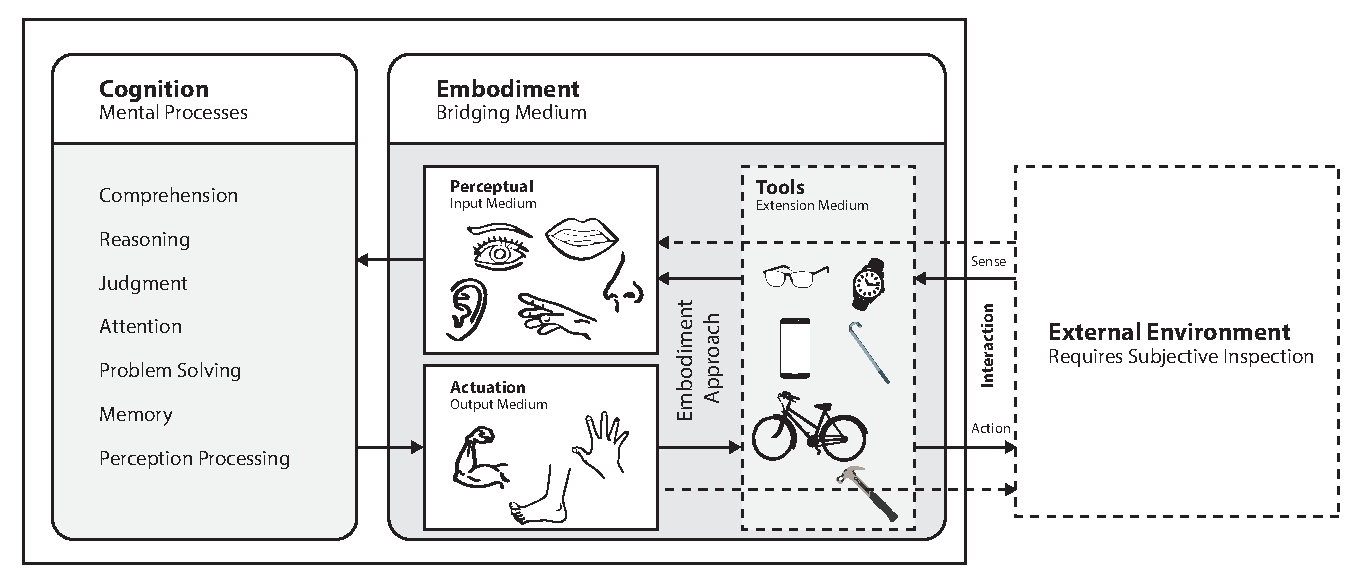
\includegraphics[width=1.3\linewidth]{figures/intro/Embodied-Cognition.pdf}}
  \captionsetup{justification=centering}
  \caption{Embodiment of tools to extend our cognition and actions into the external environment.}
  \label{fig:intro-embodiment}
\end{figure}

In philosophy and literature, embodiment has taken various definitions and concepts. MacLachlan \cite{maclachlan2004embodiment} has defined Embodiment as: \textit{the identification of an abstract idea with a physical entity}, however this base definition is rather too broad and the concept of the \textit{idea} can be self, emotion, intelligence, ...etc. Whenever this \textit{idea} is represented in a tangible matter, it can be declared as being \textit{incarnated}. Although Embodiment falls into different categories (psychology, sociology, computer science, ...etc), however, all are mainly centered around the human being, the entity with cognition and awareness. In literature and philosophy, Embodiment focuses on the relationship between our bodies and the environment surrounding it, how do we conceive information, and links to them inside-out/outside-in our mental model. Furthermore, how human cognition is shaped based on what we perceive, that is, we are what we perceive(d) and experience(d). As Shapiro describes this theme of embodiment as Conceptualization \cite{shapiro2010embodied}, our body structure defines our comprehension of surrounding world. Thus it can be viewed that human body is the interface of the mind, the channels which communicate with the outside world, and as the tangible representation of an internal idea, a thought, or an opinion when being expressed in a physical form. The expression can be a form of an act (moving a muscle group), verbal sounds (speaking), or a mediated action (through a tool, an interface, or written symbols). Likewise, perception is done through one of the five sensory organs we have: visual, auditory, tactile, smell, and taste organs. 


%describe the importance of cognitive science and embodiment here
%The standard cognitive science focuses on the idea that human perception and reasoning can be regarded as a computational model, and uses rules and symbols 

\begin{quote}
``The body is our general means of having a world. Sometimes it restricts itself to gestures necessary for conservation of life, and correlatively it posits a biological world around us. Sometimes, playing upon these first gestures and passing from their literal to their figurative sense, it brings forth a new core of significance through them - this is the case of new motor habits, such as dance.'' (Maurice Merleau-Ponty Phenomenology of Perception 1945 p.147)
\end{quote}

An ecological theory of perception was presented by Gibson \cite{gibson1966senses} which suggests that brain resonates to information presented in the environment surrounding it. That is, a structured information stimulating the sensory organs, and a brain resonating to these sensory inputs. Adding to that, Gibson's view of information acquisition insists on the fact that sensory organs should hunt for them by active involvement in the environment. 

\begin{quote}
``The perceptual systems, as it turns out, correspond to the organs of active attention with which organism is equipped... Head movements, ear movements, hand movements, nose and mouth movements, and eye movements are part and parcel of the perceptual systems they serve. These adjustments constitute modes of attention... They serve to explore the information available in sound, mechanical contact, chemical contact, and light.'' (Gibson 1966 p.58)
\end{quote}

Modern philosophers looked into the expansion of our mind using the tools that we use, representing an extension of our bodies \cite{shapiro2010embodied, malafouris2013things}. Describing the body extension phenomenon we experience when using tools \Figure{fig:intro-embodiment}. As an example, visually impaired and blind people commonly use a white cane to extend their tactile perception, and to feel objects surrounding them. Another example for entire body expansion is a bus driver, what distinguishes a professional driver from a novice one is the capability to have complete awareness of the bus he is driving, and feel it as being an extension of his body. To use the mirrors as an extension of his visual sense, driving wheel as an expansion of his motor cortex functions, and the horn as a new way of communication. The process of adapting to the tool also shape our embodiment into it, until we learn how to use it without thinking of the procedure which its operated with, as an example, when driving a bicycle \Figure{fig:intro-bicycle} we do not think of the handlebar while steering (embodied), actually when we think of how we are using it then we might lose balance and fall off (became disembodied). 


\begin{figure}[htpb]
  \centering
    \centerline{
\includegraphics[width=0.8\linewidth]{figures/intro/Bicycle.pdf}}
  \captionsetup{justification=centering}
  \caption{The use of bicycle morph our bodies, and embodies our actions through it.}
  \label{fig:intro-bicycle}
\end{figure}

Building on top of these principles of embodiment and cognition, psychologists and researchers in this field \cite{marcel1995body,gallagher2006body,pfeifer2006body,blanke2009full} began to formulate a better understanding of the body and its connection with our comprehensions of self and environment surrounding us. The cycle of interactions as input and outputs using our available modalities with the external world helps to shape a schema of our body with a mental model of it. 


\subsection{Embodied Self}

As has been discussed before, the type of representation used to reflect the inner cognitive thoughts or the medium of interaction plays an important role in communicating with the external world. The representation itself has attributes and functions that enable our cognitive functions to use and bridge with the outside world. These attributes define the level of interaction and awareness in the external environment.

In teleoperated environments, commonly operator's body is represented by a robotic form that focuses on the required operational purpose \cite{tsui2011exploring}, in which the considerations for designing the slave system is driven from the requirement of the scenario it will be used for. The design of the slave system reflects the control mechanism and the type of behavior the operator should follow to drive and operate the slave body, for example, to use a joystick to control the direction or a data glove to match slave manipulator position with hand's posture. For social and communication type of scenarios, the robotic representation is not always a necessity to be considered in the design of the system. For example, in mutual body representation, a visual representation is sufficient to transfer the state of the person located remotely \cite{ishii1992clearboard}, or for a group of people sharing the same space and collaborating remotely \cite{kunz2010collaboard} in which its possible to transfer important social aspects of communication such as eye gaze and hands gestures. Hybrid representations which both tangible and imagery representation to solve the body and social aspects as well as the physicality to manipulate remote objects were proposed. Physical Telepresence \cite{leithinger2014physical} or as commonly known as inFORM \cite{follmer2013inform} uses shape displays for interaction mediation. This type of body representation is mediating the action of the body rather than the actual spatial and physical state of it. From the user point of view, these systems do not provide a full sense of immersion, but rather as being looking through a window or medium which they perform their actions within rather than being the medium.

Virtual representation of the body has enabled to overcome the physical constraints of the representation. Ogawa et al. \cite{ogawa2012reachable,ogawa2016metamorphosis} proposed a user interface which extends hands interaction by deforming the visual feedback of user's arm, such as extending its length to reach far objects. Asai et al. \cite{asai2016extendedhand} used this type of interaction for people with a mobility impairment to easily point to physically far surfaces. The virtual representation has also enabled social researchers to investigate the effect of changing body skin color or race to a different one to decrease the racial bias against dark-skinned people \cite{peck2013putting,rosenberg2013virtual}. The study highlights the importance of multisensory correlations to induce the illusion of body ownership toward the virtual body, which relates to the level of embodiment the participant's experience. Within the same context, \cite{maister2015changing} showed that experiencing a body with superpowers (as being a superhero in sci-fi) to fly in a virtual environment based on embodied actions, like acting as Superman to fly, would lead the participants to engage in a pro-social activity to help others in need after finishing the experience. Further investigations on reproducing the illusion of virtual body ownership for non-humanoid creatures has been studied in \cite{lugrin2015anthropomorphism}. Probably the virtual bodies are the true alchemy of embodiment.


%%%%%%%%%%%%%%%%%%%%%%%%%%%%%%%%%%%%%%%%%%%%%%%%%%%%%%%%%%%%%%%%%%%%%%%%%%%%%%%%%%%%%%%%%%%%%%%%
\section{Body Schema \& Modalities}
\label{sec:intro-bodyschema}

\begin{figure}[b!]
  \centering
	  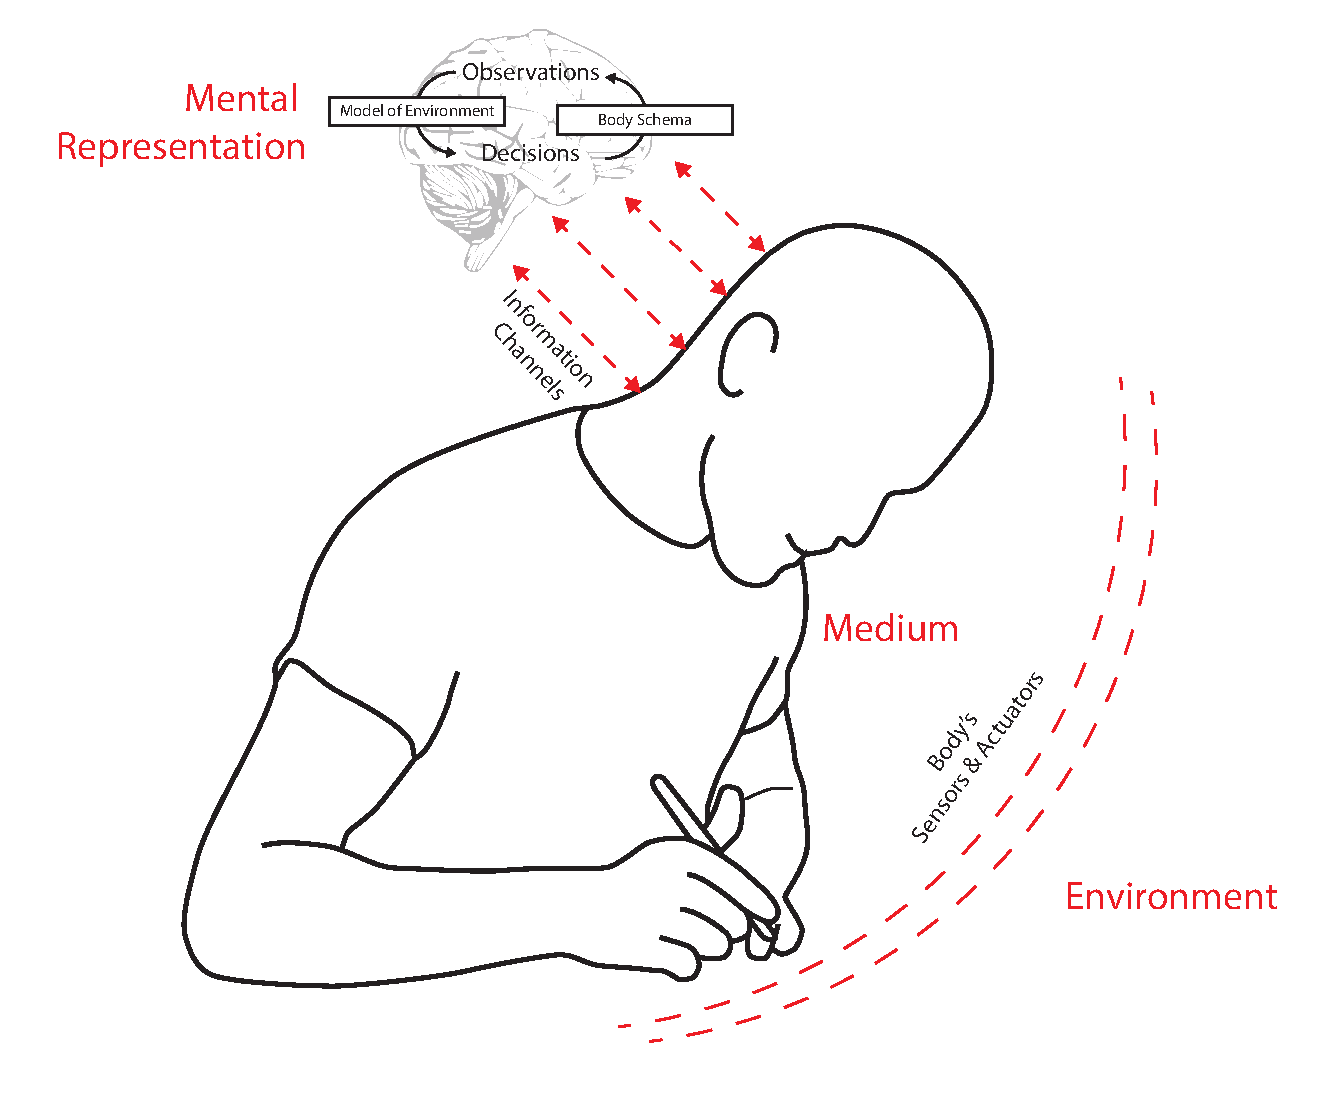
\includegraphics[width=0.75\linewidth]{figures/intro/BodyInteraction.pdf}
  \captionsetup{justification=centering}
  \caption{Body schema is a constant internal process representing the medium of interaction (body).}
  \label{fig:intro-bodymodel}
\end{figure}

Body Schema involves aspects of both brain processing and body peripheral (Proprioception signals, sensory signals), and it is considered as a collection of processes that stores the posture of the body and relationship of body and its representation. When the body state became in motion, the body schema updates unconsciously according to that motion \cite{holmes2004body}. A mental image maintains a constant representation of the body while a task is being carried on \Figure{fig:intro-bodymodel}. The observations/decision loop which is unconsciously updating our mental representation relies mainly on the information channels that interact with the body. In some sense, its possible to represents the body as being a medium between the internal mental image, and the surrounding environment in which the body is located at, and at which the task is being performed in. 

The idea of the body schema and the mental image of the body has been derived from philosophical and empirical perspectives. Aristotle in his book (On The Soul, II) referred to the soul as being the form of the physical body, which perishes together with it at the death. And according to Spinoza (The Ethics, II) said the soul is the \textit{idea} that the body develops of itself. In a modern term, the \textit{idea} is simply a mental representation, more precisely, a self-representation. Gestalt properties, such as body shape, are rather global properties of the entity, and thus the body schema or the self-representation is being a neural mechanism to represent exactly such global properties. In a modern philosophy, Matzinger \cite{metzinger2007empirical} has presented that the body and self can be a plastic representation and highly context sensitive. He referred to the self-representation with the concept of ``Self-model'', which is a process driven by a series of cross-modal interactions from the several sensory channels in order to define the image of self and body. For example, in the rubber-hand illusion (RHI) \cite{botvinick1998rubber}, the sensation of being stroked with a prob is integrated with visual and kinesthetic feedback in order for the brain to constructs a matching proprioceptive map between the subject's mental image of his body and what he perceived from the sensory channels. As a result, the subject's mental image of the body ownership is redefined and would then believe the rubber hand is part of his body. This illusion is extended to modulate the body schema to perceive a third arm as being a part of the body \cite{guterstam2011illusion}.

By considering \textit{the body as a medium for interaction}, then its possible to create a proxy that maps the sensors and actuators of the body into a different representation. In Telexistence, previous research showed the possibility to transfer body awareness using a remotely operated avatar matching operator's body schema \cite{fernando2013design}. A visual-kinesthetic transfer model is defined to create the sense of bodily presence and ownership toward the remote representation. And fundamental elements for presence, such as vision matching, real-time control and operation, and tactile feedback, are important elements in creating such a schema transfer model. By maintaining such baselines for presence, and defining a top-level model to remap the other modalities, it would become possible to redefine body schema while preserving the sense of ownership toward the alternative representation.


Within the scope of this thesis, Embodiment emphasizes the role of the body in defining and shaping the mind and its cognition through the sensory-motor skills being performed, and the sensory-perceptual inputs being perceived. That is, the body is being the medium and the interface of the mind.

\subsection{Isolated Modalities}

A modality can be considered as a single independent channel of sensory input/output between human and the surrounding environment. As in our daily interaction, we rely on cross-modalities to have a clear comprehension of the tasks we involved in. Human body physical structure imposes tight coupling of these modalities, and our mental representation is mapped to this tight coupling. However this tight coupling can introduce an overlapping information, and some of the sensory inputs are not necessary for the task being involved with or would result in sensory distraction between the various sensory modalities.

%\begin{comment}
Isolating the involved modalities for a specific task would enhance the operation and achieve a higher sense of \textit{attention} by reducing non-relative sensory and perceptual information (distraction).

\begin{quote}
``Everyone knows what attention is. It is taking possession of the mind, in clear and vivid form, of one out of what seems several simultaneously possible objects or trains of thought. Focalization, concentration of consciousness are of its essence. It implies withdrawal from some things in order to deal effectively with others, and is a condition which has a real opposite in the confused, dazed, scatter-brained state which in French is called distraction, and Zerstreutheit in German.''  (William James - The Principles of Psychology Vol. 1 1980 p.404)
\end{quote}

In his definition of \textit{Attention}, James highlights the role of isolation of a sensory stimulus through the concentration towards it in order to effectively engage in or observe from a certain action.

\begin{comment}
As an example, libraries in a sense removes the distracting auditory noise and ban them so the scholars in the library can focus or immerse themselves in reading. Similarly in cinema theaters in which also the customers tend to concentrate and engage with the provided contents.
\end{comment}


\begin{figure}[t!]
  \centering
	  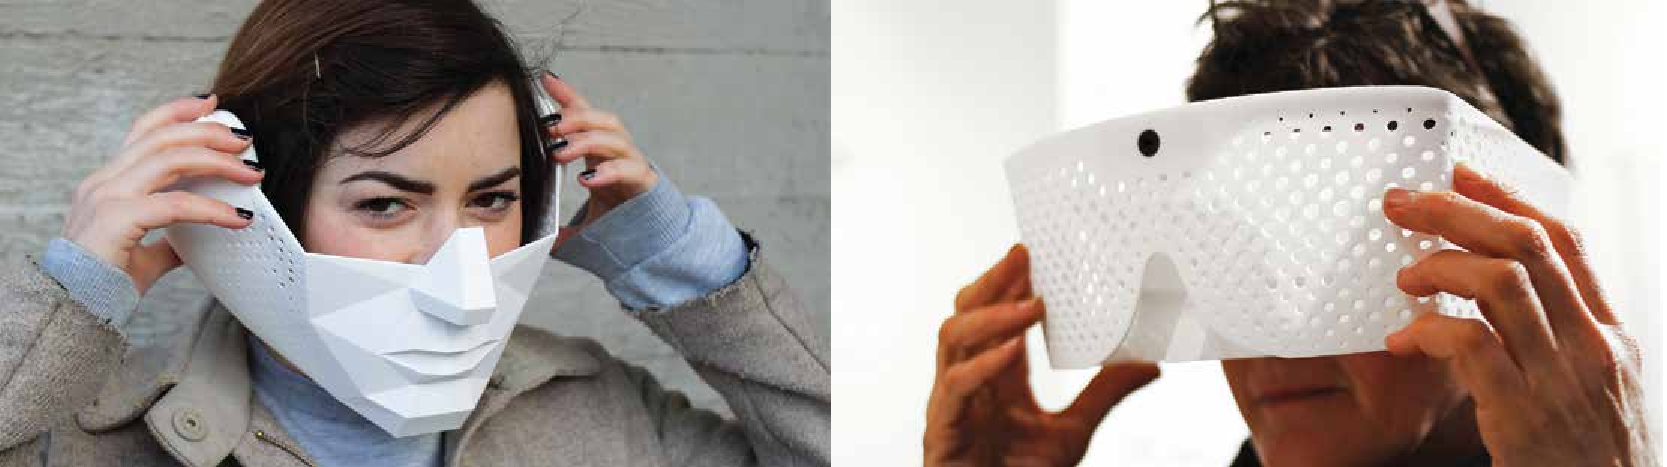
\includegraphics[width=1\linewidth]{figures/intro/Eidos.pdf}
  \captionsetup{justification=centering}
  \caption{Enhancing perceptual modalities using wearable devices. Eidos Audio (left), and Eidos Vision (right). }
  \label{fig:intro-eidos}
  \text{\footnotesize Photo \copyright\xspace Eidos (2012).}
\end{figure}

Abstracting the individual modalities, based on their function and type of information they carry, would assist the design and use of digital tools and media to enhance them individually, and then provide their contents back to the user through feedback devices. Eidos \cite{tim2012eidos} shown in \Figure{fig:intro-eidos}, illustrates the possibility of controlling our individual senses and adjusting them separately reducing other distracting information. Isolated modalities based design helps enhancing individual modalities functions, or even achieve supernatural capabilities such as augmenting visual perception \cite{koizumi2012stop}. 


\subsection{Body Ownership}
In order to establish that our perception of body and self can be altered via modifications of our sensory modalities and embodied representation, psychological studies and empirical evidence are required to support this claim. Previously we discussed the phenomena of rubber hand illusion which can create a strong sense of ownership to an artificial body based on the cross-modality experience of vision and haptic feedback. That example showed how the perception of body part ownership can be altered through external stimuli. 

In a contrasting example of altering the sense of body ownership: the phantom limb sensation \cite{melzack1992phantom}. In this phenomena, a person perceives a missing arm or leg as still existing regardless of the fact that it's being not physically present. That is, their mental image of their body still poses the perception of the capability of moving the limb, the proprioception feeling of its posture, but without visual or tactile feedback from the missing limb. This inconsistency of perceptual feedback with the internal mental image of the body causes what is called phantom limb pain. In one of the previous studies on the phantom limb pain treatment, the visual illusion of missing limb was 'resurrected' back to the patient using a mirror setup \cite{ramachandran1995touching} in which the patent sees his functioning limb in the location of the missing limb. An illusion of kinesthetic sensation emerged during the trials, even when the experimental used his hand instead of the patent hand to induce this sensation. 



%Where Am I by Daniel Dennett 1981
%Chapter 3 discusses further details about \ProposalKeyword for body mapping using modalities input/output channels. Also, a Telexistence Toolkit is proposed as a proof of concept. The toolkit provides hardware set which can be used along a meta-modeling software for defining the relationships between operation and representation.

\subsection{Modalities Substitution}

Brain plasticity and adaptability to modulate sensory feedback and restructure the perceptual awareness has been widely investigated in psychology and neurology. A subset of this area of research is modalities or sensory substitution. This research involves the study of the effective sensory modalities that can be used to replace another one. Thus the research involves the study of meaningful conversion of the information from one modality to another, and the representation used to deliver the newly converted information.

In neurology area of study in sensory substitution systems, a person who lost a certain sensory due to peripheral damage still has the capacity to sense within his brain structure. For example, for a blind person, the peripheral sensory system (retina) is not functional which results the fact of blindness is still has the capacity to ``see'' from neurological perspective unless if the visual cortex of the brain is damaged. Similarly for those with positional orientation and balance disorders (the vestibular apparatus), or deaf due to sound transduction damage in the ear (the cochlea). Previous work \cite{bach1972brain, bach1995nonsynaptic} found that the input from a sensory substitution system can stimulate the brain regions which lost its sensory peripheral. 

\begin{figure}[b!]
  \centering
	  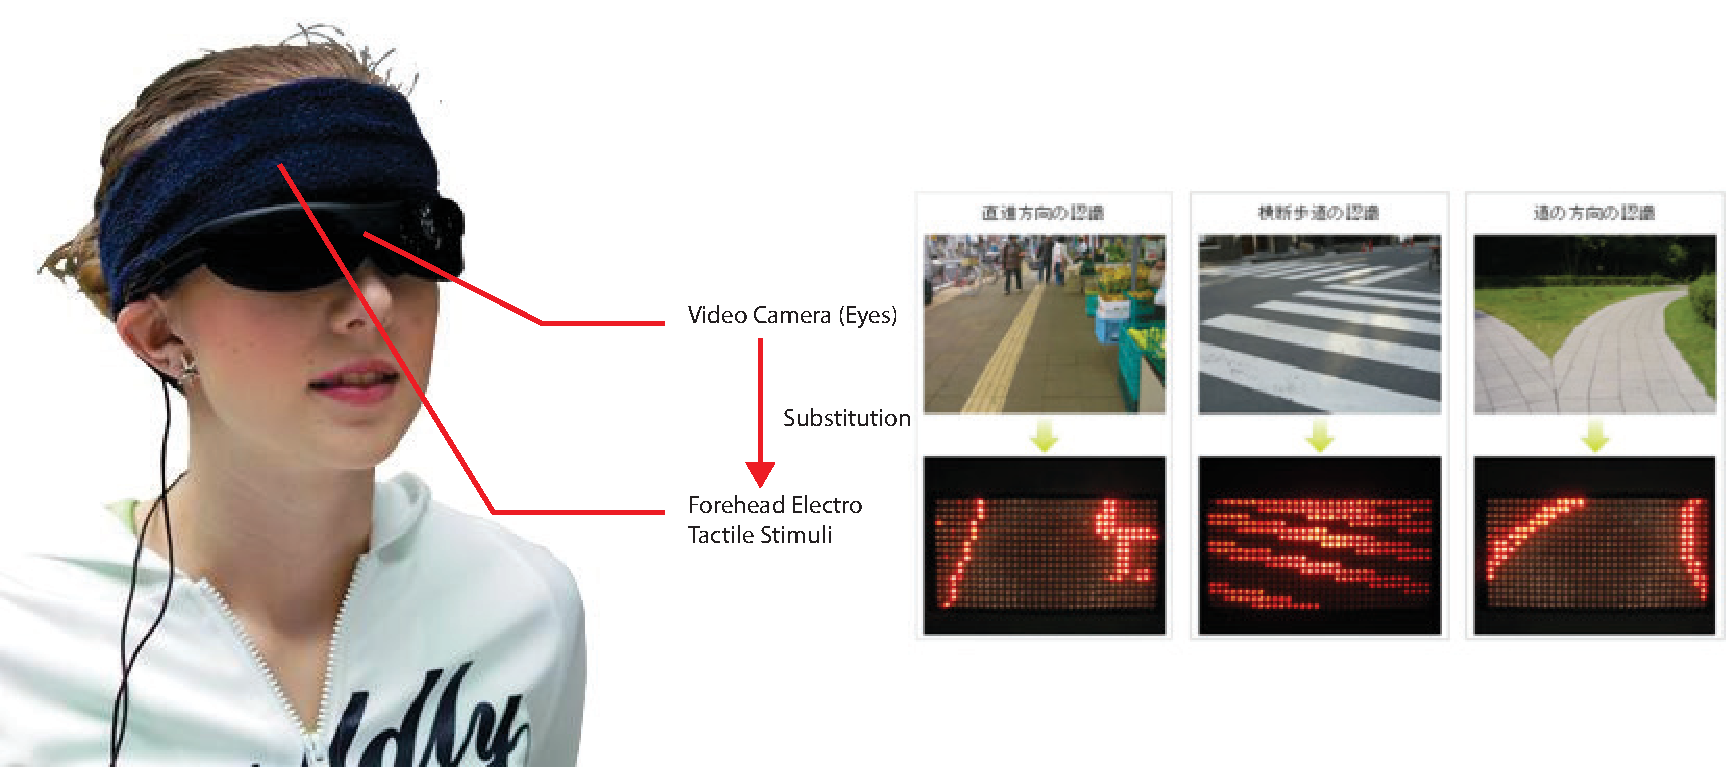
\includegraphics[width=1\linewidth]{figures/intro/SSD.pdf}
  \captionsetup{justification=centering}
  \caption{Visual sensory substitution using tactile feedback }
  \label{fig:intro-SSD}
  \text{\footnotesize Photo \copyright\xspace AuxDeco, Inc (modified from original)}
\end{figure}

Sensory substitution devices (SSDs) have been commonly used as means of non-invasive methods to restore a certain sense of the surroundings. SSDs are generally divided into two main variations: visual-to-tactile substitution devices that translates optical information into tactile stimuli, and visual-to-auditory substitution devices that convert sound into an audio wave. Widely used is the tactile based SSDs to restore the visual modality for blind people, and as one of the earliest examples of such tools is the white cane which still being used until now by blind people (recently proposed EyeCane \cite{maidenbaum2014eyecane} augmenting the traditional white cane). Braille is another commonly used SSD to provide tactile amount of information of written symbols. White et.al \cite{white1970seeing} developed a tactile SSD that converts the optical images captured by a camera into an input to an array of solenoid vibrators located on the back of the user to induce visual information through tactile sensory channels. Commercial products that use electro-tactile stimuli to substitute the visual modality has been also introduced previously, AuxDeco by EyePlus-Plus Co. Inc \cite{auxdeco} uses forehead as input surface for the visual information, while BrainPort by Wicab Inc. \cite{brainport} uses the tongue. The other spectrum of SSDs used auditory feedback. As one of the very first SSDs is ``Ultrasonic Eyeglasses for the Blind'' proposed by Leslie Kay \cite{kay1973sonic} which is a biomimicry glasses that uses ultrasonic sensors to measure the distance and the geometry of the objects, and produces auditory tones that vary in frequency depending on the distance. More recently, the vOICe by MetaModel Inc. \cite{vOICe} uses the audio modality as a substitution to the vision by converting visual stimuli into musical notes. Other variations of vision-to-auditory approaches to transform the image data have been widely investigated \cite{meijer1992experimental,capelle1998real,hanneton2010vibe} which are not only used for visually impaired people, but also as approaches to transform visual information to meaningful auditory information.


\begin{comment}
%Substitutional Reality, not clear if it links in this context
A recent variation of perceptual substitution is the reality substitution. Substitutional Realities (SR) was first coined by Suzuki et.al \cite{suzuki2012substitutional}, in which a proof of concept system was developed. As in conventional modality substitution systems discussed before, the SS system is used to replicate the input of a lost modality using a different sensory peripheral, in SR the sense of reality and time is being substituted with an alternative pre-recorded visual feedback input. The approach of SR is to blend in and out the real-time and past recording in a controlled condition which might involve physical interactions between the experimenter and the participant in real-time period convincing the participant of the physical presence. The pre-recorded visuals is done from the same point of view of the participant's eyes in omni-directional manner, thus when the blending with the past occurs, the participant maintains consistent flow of information along his head motion. Under controlled conditions, SR proved that the sense of presence is possible to alternate using single modality substitution. The participants expressed high level of confusion of whether what they see is happening in real-time within their spatial bounds. Derivations of SR has also been proposed, Reality Jockey \cite{fan2013reality} in which the focus was on auditory modality substitution, and \cite{simeone2015substitutional} which uses physical/virtual space substitution to enhance the bodily experience of presence in virtual reality applications. Blended Reality \cite{kevin2017blended} expands on SR topic to address the variations of presence substitution in terms of time, space, and modalities.
\end{comment}

\subsection{Body Morphology}

\begin{figure}[b!]
  \centering
    \centerline{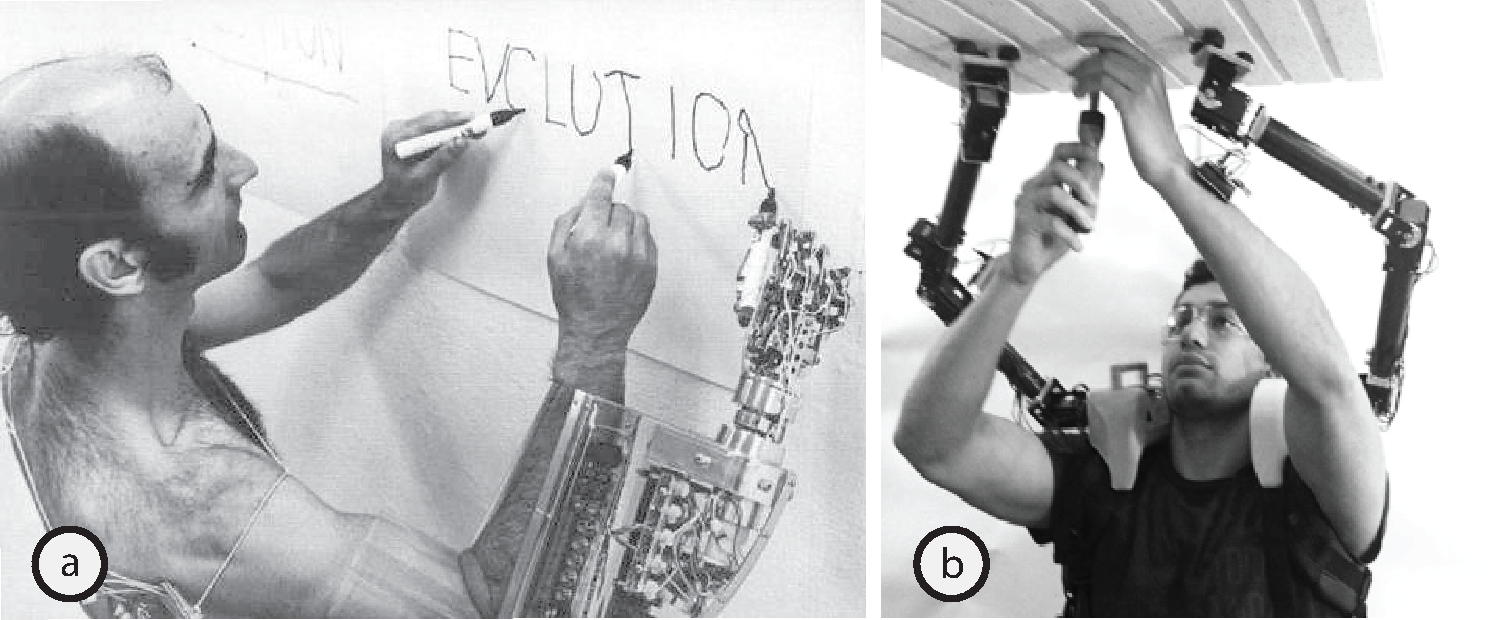
\includegraphics[width=1\linewidth]{figures/intro/BodyExtension.pdf}}
  \captionsetup{justification=centering}
  \caption{Body physical morphology using additional limbs. (a) Stelarc Third Hand motion is driven from body muscles, where (b) MIT's Supernumerary Robotic Limbs (SRL) action are application driven.}
  \text{\footnotesize Photo \copyright\xspace (a) Stelarc, and (b) MIT Federico Parietti.}
  \label{fig:intro-bodyext}
\end{figure}

To overcome the rigidity in physical constraints our body schema constitutes, first a digitization of our body's sensory and actuating modalities is needed. The conversion from analog/physical representation into a digital form would provide the required flexibility to remap, augment, and alternate what we observe and how we operate. The process of digitization of the body can be done using sensors to track the different types of actuation body presents, and perceptual proxies devices which produce different types of sensory feedback to the body. As seen in the previous section, the sensory feedback can be modulated or substituted before providing it to the user's body in order to overcome a certain disability or to augment a modality. Such process will be referred to as modality transfer.

Modality transfer can be seen in two types: Local schema transfer when the medium of interaction is spatially located along the body so its modalities are cooperating with the alternative modalities used to shape the body schema. And remote schema transfer when the medium of interaction extends spatially into a different location, thus the cognition relies completely on the used representation to communicate with the environment. 

In local schema transfer, it is possible to induce new body schema when we use tools that, for example, shift the function of the modality in a constant manner. For example, when using a pen for writing, the pen becomes an embodiment of an object with the functionality to point, write, and touch. When we adapt to the use of the tool, it becomes transparent and a part of our new body schema. Robotics has been used also to reshape our functions in an embodied or assistive manner \Figure{fig:intro-bodyext}. Stelarc Third Hand \cite{kac1997foundation} was one of the first ``successful'' trials to embody an extra robotic prosthesis to his biological body. The prosthesis was physically strapped into his right arm, but had functions to grasp, pinch, and rotate its wrist. The arm is considered as being embodied because its motion was driven from his bodily functions, that were EMG\footnote{Electromyography which records muscle activities using electrodes placed on a relevant skin surface.} signals from his legs and abdomen. The EMG signals acted as a real-time digitization of some functions of his body which served to be a transparent channel communicating with the prostheses. This bodily driven control allowed him after many years of use to adapt this arm to his body schema, and to operate it as an extension of his body \cite{stelarc1980thirdhand}. On the other hand, other types of tools are considered as assistive rather than being embodied with the human body, such an example is the Supernumerary Robotics (SR) \cite{llorens2012based,bonilla2014robot, parietti2014bracing, wu2014bio}. Such type of SR systems are designed to work side by side with a human operator in a coordinated manner, it has an independent behavior when performing the tasks to optimize the operation which the human is performing through independent observations and reactions. Thus its motion is not driven by direct bodily actions, but rather from the task's context, which means the arms could be considered as a separate entity disembodied from the human operator.

\begin{figure}[htpb]
  \centering
	  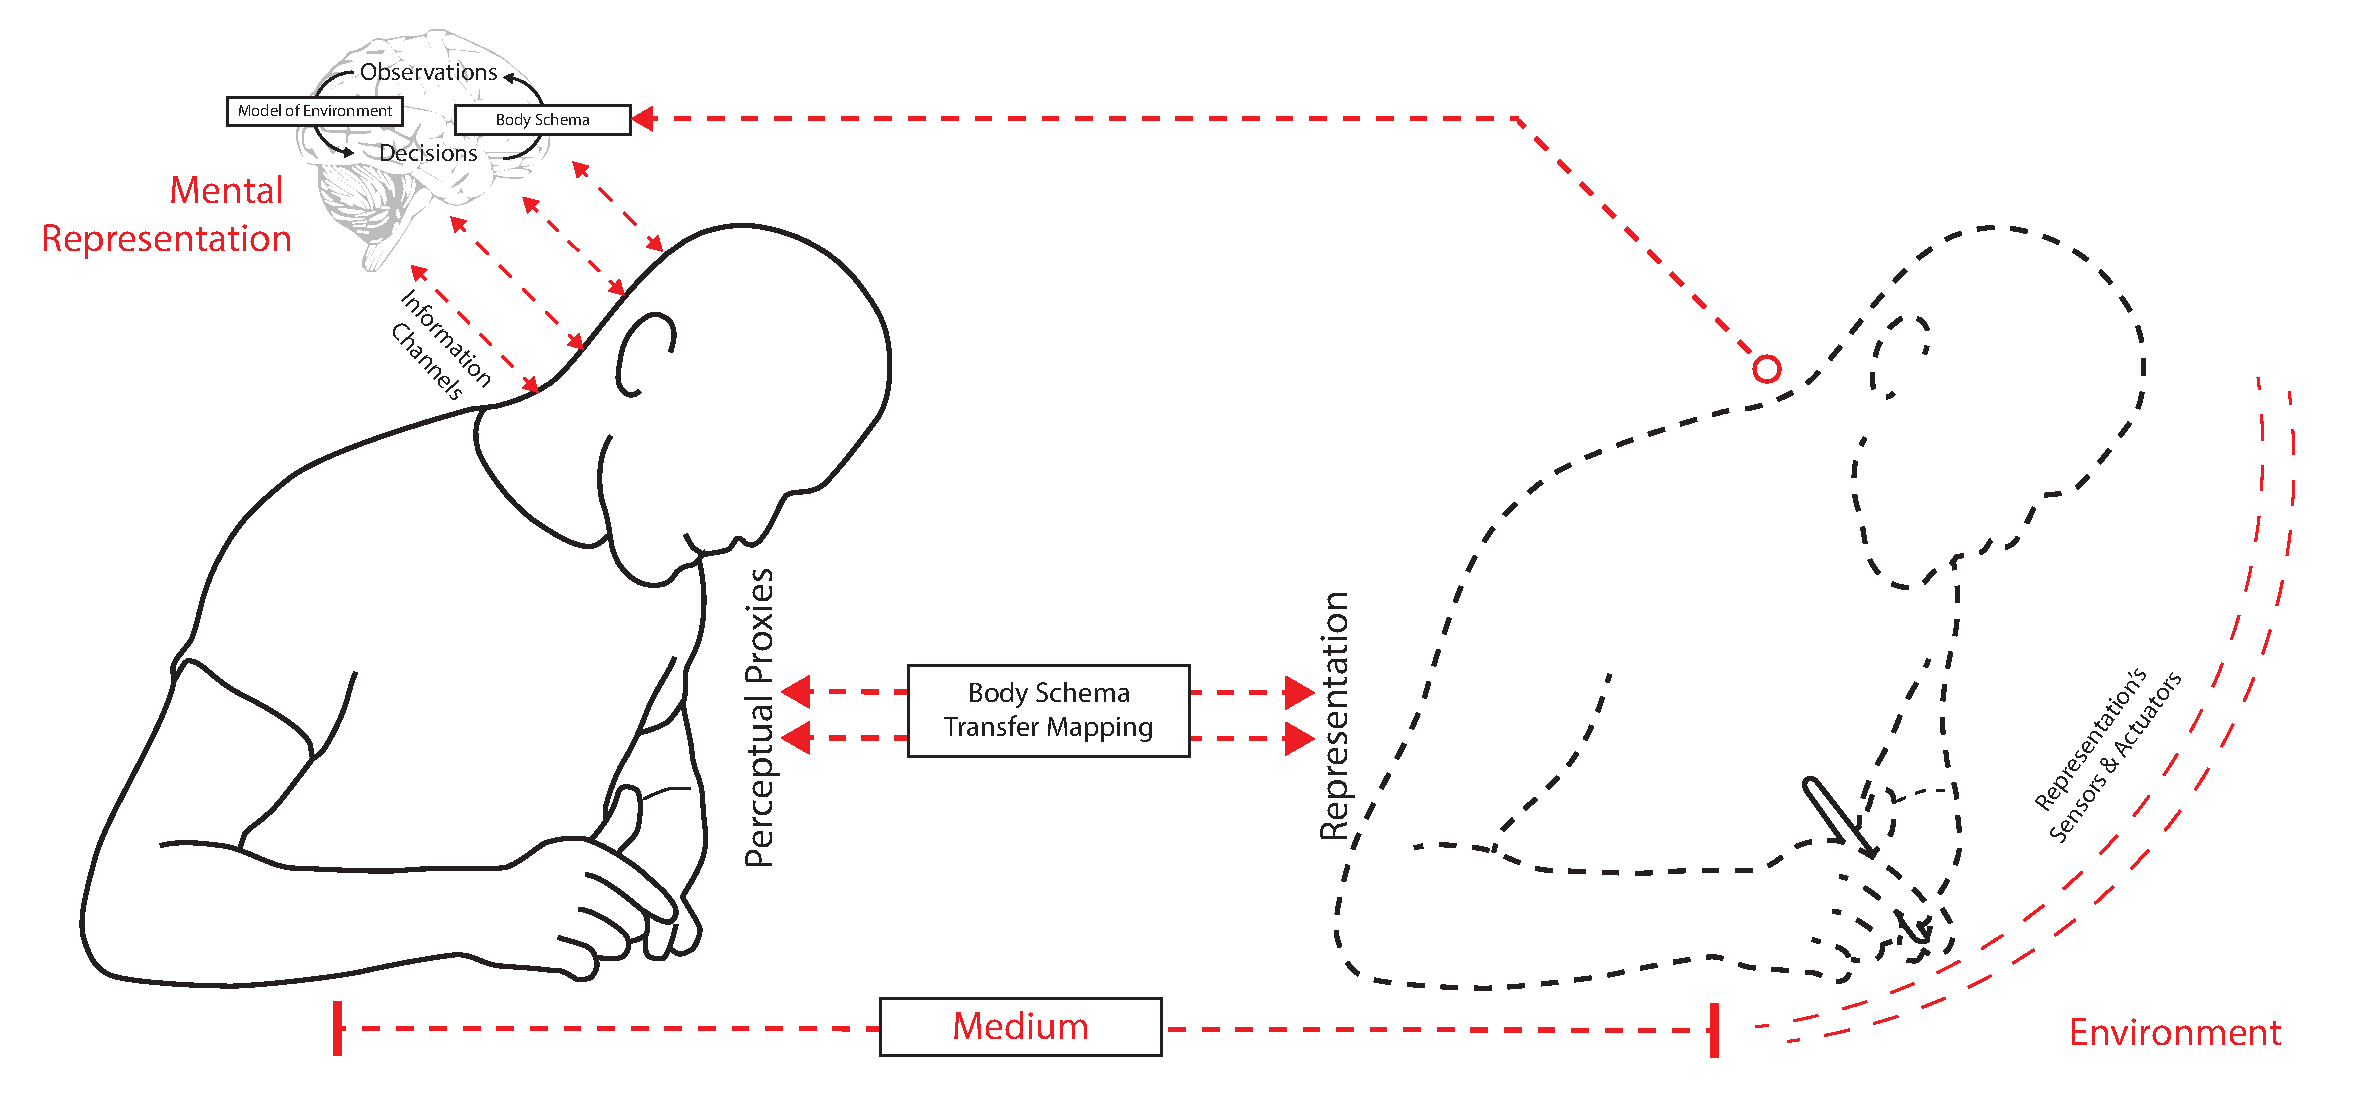
\includegraphics[width=1\linewidth]{figures/intro/representation.pdf}
  \captionsetup{justification=centering}
  \caption{An overview of the process of digitizing human body perception, and extending the medium of interaction (human body) into an alternated representation. Body modalities are transferred into an alternative representation.}
  \label{fig:intro-digitalRep}
\end{figure}

For remote schema transfer, the process of body schema adaptation requires the modalities to be transferred from one location to another by digitizing their functions so its possible to capture and reproduce them from one side to another. \Figure{fig:intro-digitalRep} provides an overview of the process of digitizing body schema, and transferring it from an alternative representation into the body via perceptual proxies. Body schema transfer mapping block acts as a definition for the process of real-time updating the representation with the human body using the digitized sensory channels. Work in telepresence and telexistence derives similar approach for creating a sense of presence in a remote environment for teleoperation purpose. These approaches, as will be discussed in the next section, transfer the body modalities from one location to another to stimulate the sense of remote presence.
%Previous work showed that our mind has the plasticity to continuously shaped and re-shaped to new body representations, for example, to embody different body \cite{peck2013putting}, or to alter the physical properties of the body \cite{rosenberg2013virtual}.  



In conclusion, in order to alternate body schema, there should be a consistency of sensory inputs regardless of the physicality of the observed body or the representation, thus maintaining the sense of ownership. Also, to preserve the sense of agency towards the body, the observations from the body (e.g. movement) should be correlated with the actions of the user. 


%%%%%%%%%%%%%%%%%%%%%%%%%%%%%%%%%%%%%%%%%%%%%%%%%%%%%%%%%%%%%%%%%%%%%%%%%%%%%%%%%%%%%%%%%%%%%%%%
\section{Presence Augmentation \& alteration}

In this section, discussion about related work in body presence augmentation and alteration. Work in Telepresence, Telexistence, and spatial awareness are described showing the impact of such means to expand body's limited perception and actions. 

\subsection{The Essence of Presence}

Presence is the state of awareness of body and its surroundings. Enhancing the state of presence or altering it is to change the physical constraints or to convince the mind of being at a different state than what the body physically is. Kim \cite{kim1996effects} highlights on that as ``feeling of being a part of the phenomenal environment created by television and not being a part of the physical environment surrounding the viewer and the television set''. Similarly, with the use of virtual reality tools, it's possible to lead the mind into a ``suspension of disbelief that they are in a world other than where their real bodies are located''\cite{slater1993representations}. The state of presence is a flexible term that can stretch over time and space, as well as the form of body perceiving the various sensory modalities which develop the understanding of where and how the body is located at. 

In physically teleoperated environments, several work and research discussed the requirements to provide a physical presence to operate and to be embodied (as being part of the remote location). Minsky \cite{minsky1980telepresence} proposed telepresence systems that function to provide ``feeling like you are actually 'there' at the remote site of operation''. Minsky highlighted the role of teleoperated systems to empower the functions of human operation and labor to perform an effective operation for the tasks at hand. The essence of providing the sense of transferring body awareness to remote slave system was proposed by Tachi in his paper on Telexistence systems  \cite{tachi1985tele}.  ``a system that at the remote control-site a human operator can perform remote manipulation tasks dexterously with the feeling that s/he exists in the slave anthropomorphic robot in the remote environment.'' which is referred to as Tele-existence system (or Telexistence) under the condition of  ``real-time sensation of remote presence''. This definition provided a requirement of the subjective experience of body presence ``...perform remote manipulation tasks dexterously with the feeling that s/he exists in the slave...''. The requirement of mapping and matching the state of the body between the human operator and the slave system creates a strong sensation of agency and ownership. Rheingold \cite{rheingold1991virtual} described Telexistence systems as a ``form of out-of-the-body experience'' once he looked at himself through the slave system. Telexistece systems can be viewed as a way of presence augmentation since the body's physical constraints are extended over distance, and the effect of manipulation and perceiving can be done remotely. The usage of mediated technologies can help to reproduce the sense of presence, and thus can be a mean to enhance and alter this sensation.

State of presence can also be stretched to non-physical environments. Virtual presence is usually regarded to the state of being in a non-tangible space which is being represented by digital means. Sheridan \cite{sheridan1992musings} created the distinction between physical and virtual, in which physical presence is characterized as ``physically being there'' while virtual presence as ``feeling like you are present in the environment generated by the computer''. The master/slave system of Telexistence also proposed to operate under virtual environments as if being in a physical one \cite{tachi1991tele}, extending the concept of presence into virtual, non-physical spaces.

\pagebreak
\subsection{Connected Awareness}


\begin{shaded}
\begin{quote}
\textit{
\centering{\textbf{The story of ``Waldo''}}\\
%http://cyberneticzoo.com/teleoperators/1942-waldo-and-waldoes/
``Waldo'', a fictional novel by Robert A. Heinlein 1945 \cite{heinlein1942waldo}, tells a story of a mechanical genius who lived his entire life in a self-imposed exile: his own body. Struck with a neuromuscular disease (myasthenia gravis) in which it locked him inside the shell of his weak body, he was capable to develop dozen of mechanical hands (called as Waldo F. Jones Synchronous Reduplicating Pantograph) which are operated via sensory devices attached to his hands, and extend his body and enable him to amplify his weakened muscular strength. These mechanical hands were depicted as in various sizes which can be as small as micrometers in span allowing him to micro-manipulate, and all the way up to six meters from finger to thumb in size allowing him construct buildings and facilities while imitating his hands motion and actions. Despite of the fact of being crippled in his weakened body, Waldo considered himself as a superior to humanity since his augmented skills and his body extensions enabled and empowered him to do far more superior tasks than what a fully functional human can do. 
}


\end{quote}
\end{shaded}

The story is considered as one of the very first original novels which highlight the effect of technology and tele-body-representations to augment the motor skills of our bodies. Also, it highlights the effective adaptation of connected bodies and awareness to amplify our cognitive skills and enhance our physical capabilities. 

Thanks to the never-ending expansion of interconnected networks and Internet, the boundaries of location and space has expanded from local to a global scale and created a true ubiquitous information accessibility. Mark Wiser\cite{weiser1994ubiquitous} introduction to Ubiquitous Computing helped to create a new paradigm of information accessibility and networked computational design. These technical innovations in network media and information accessibility opened a wide door for the emergence of digital-based Teleconferencing and Teleoperation tools at a wider scale compared to the older analog-based media transmission. These tools provided the capability of transporting human beings virtually from one place to another to get involved in a remote discussion, or to transport his skills for solving remote tasks. 

\begin{comment}
Back in 1980s, Susumu Tachi \cite{tachi2016telexistence} \& Marvin Minsky \cite{minsky1980telepresence}, both scientists \&  visioners from the east and the west proposed the means and concepts of the tools and medium which human operator can use in order to have the awareness of the distant location. There is a fundamental difference between the concepts proposed by Minsky (Telepresence) and Tachi (Telexistence). The former concept focuses on the tools to operate remotely and on the quality of remote task, however, the latter one addresses cognitive and awareness related factors for the quality of operation and sense of presence. Each of the previous teleoperation approaches has a different aim \Figure{fig:intro-tele}, the former is task transfer oriented approach, while the latter is body transfer oriented approach. For the human operator, it helps to have a sort of Teleportation from one place to another instantly and to avoid any risk of exposing his biological body into a hazardous environment which the avatar can be located at. Also, it transports the knowledge and expertise of the user instead of using Artificial Intelligence based robots. 
\end{comment}
%require to cite a work about self-consciousness \cite{lenggenhager2009spatial} before talking about telepresence systems

\begin{figure}[!ht]
  \centering
  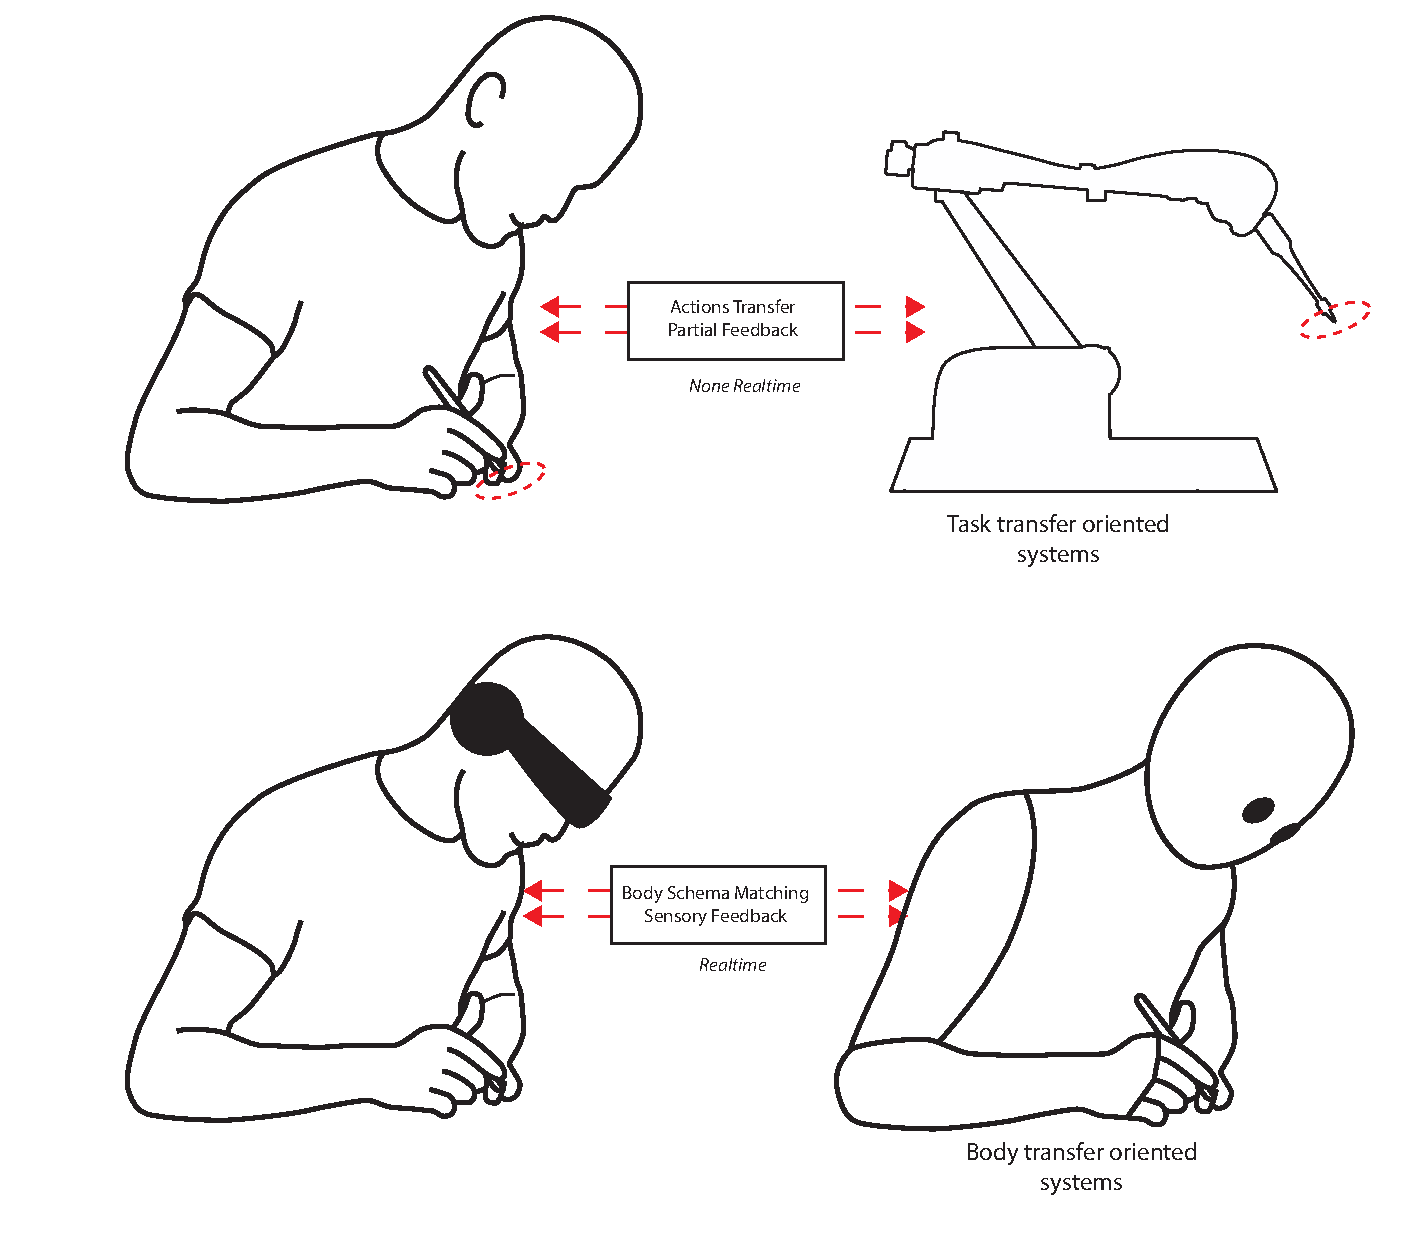
\includegraphics[width=1\linewidth]{figures/intro/Teleoperation.pdf}
  \captionsetup{justification=centering}
  \caption{Task vs Body transfer oriented systems. }
  \label{fig:intro-tele}
\end{figure}


Basic teleconferencing tools, such as Polycom video conferencing \cite{rodman2004polycom}, Skype, and Google Hangouts provide an easy to use means to connect remotely, however they lack to represent the physical attributes of the operator, and rather have limited number of modalities that are engaged (commonly video/audio feedback). The other paradigm aside from the basic teleconferencing tools could be categorized to Telepresence and Telexistence technologies \Figure{fig:intro-tele}. Each of these addresses different type of cognitive transfer, the prior is task transfer and the latter is body transfer.

Telepresence systems emerged to the market and gave higher levels of flexibility for operation and representation, such as MeBot \cite{adalgeirsson2010mebot}, Kubi \cite{kubi2013}, and Double Robotics \cite{robotics2015double}. These systems would allow motion and teleoperation and even can transfer non-verbal cues via robotics hands, or facial expressions \cite{misawa2013livemask}. Telepresence systems, in general, can be referred as task transfer-oriented systems, which focuses on the use cases of the system instead of the full embodiment of the operator.

\begin{figure}[htpb]
  \centering
  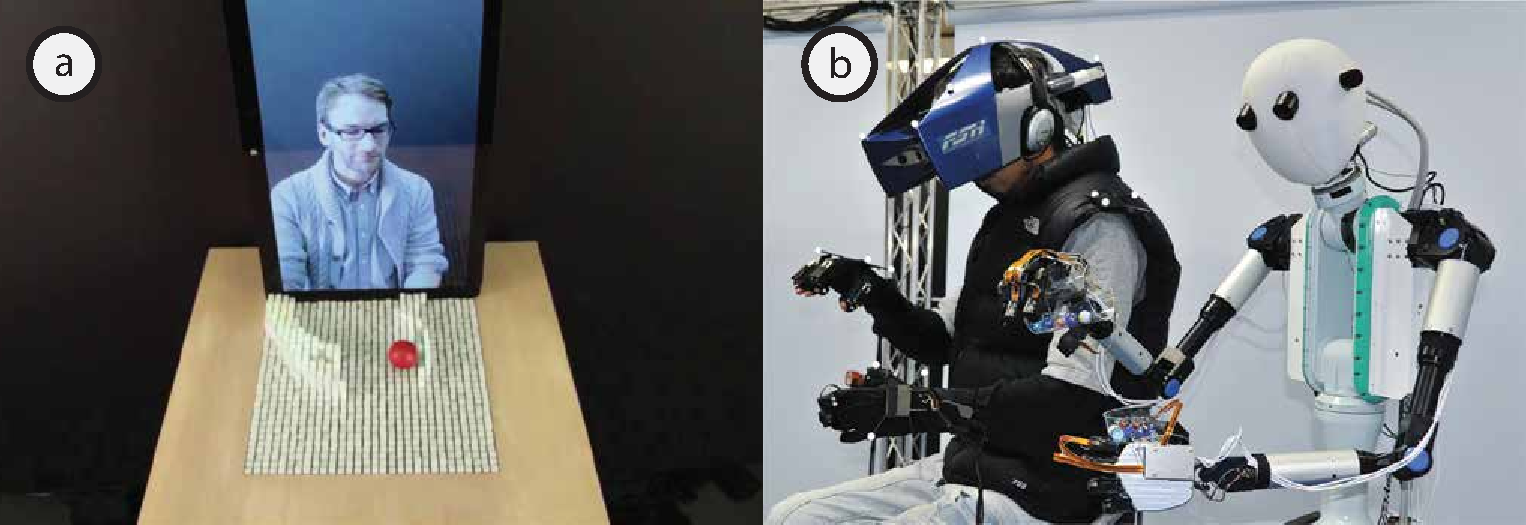
\includegraphics[width=1\linewidth]{figures/intro/TeleTech.pdf}
  \captionsetup{justification=centering}
  \caption{Embodying teleoperation technologies (A) inFORM as an example of Telepresence systems, and (B) Telesar 5 as an example of Telexistence systems.}
  \label{fig:intro-tele}
  \text{\footnotesize Photo \copyright\xspace (a) MIT Tangible Media Group, and (b) Tachilab.}
\end{figure}

In Telexistence related applications, an avatar that represents a substitute representation of human body using robotic systems and digital forms, the human operator can remotely access and have immediate control and real-time feedback sensation from the remote surroundings as if the operator is actually located there. Although current Telexistence systems \cite{tachi1985tele,tachi1990tele, hasunuma1999development,kawakami2005telesarphone,watanabe2007torso,fernando2012iros} provide a partial representation of the human body, however, they achieve a strong sense of self-consciousness and sense of presence in the remote place, which Telepresence systems lack.

%Both Telexistence and Telepresence are solid implementations of that novel.

In some sense, we can say that both Telepresence and Telexistence systems are a one-to-one mapping of the user to his avatar (best case when a full body representation is achieved). Based on this definition, although avatar representation provides enhancements to the human operator and overcomes several difficulties that direct human operation cannot serve, these methods of direct one-to-one mapping has upper bounds of what an augmented human can do. The question is, what happens if a physically disabled person tried to use such systems? As its a direct one-to-one mapping, the disability will also arise in the representation too. In Waldo's case, his body was weak but not disabled, and his hands were still being represented as direct one-to-one mapping with his waldos. Without his basic motor skills, he would not be able to operate the body amplifiers he invented.


\subsection{Presence Embodiment}

Media interfaces are progressively growing to embody us within it, affecting our sensations of physical presence, social presence, and self-presence inside. This progression in telecommunication technologies creates a tighter coupling between the body and the interface, in which the body becomes a part of the physical space and the cyberspace. This progression creates an adaptation between the body and the interface \cite{biocca1997cyborg}. Adding to that, research in Virtual Reality and cognition showed that sense of presence can be provided through technical means and psychological experiences \cite{riva2006communication}. Technological means are the physical representation of sensory organs, such as stereo vision (eyes), binaural audio array (ears), tactile system (touch), ..etc. The psychological experiences define the relationship between the technological means and the human body. Thus by altering both the means and the experience, sense of presence can be altered or enhanced, while maintaining the seamless experience of presence, or of being there.


\subsection{Beyond Presence}

The question of the possibility to leverage what our bodies can perform, or expand the perceptual capabilities of our visual, auditory, and tactile modalities has been a focus in human augmentation research area.

Recent systems were introduced to share the presence, and can be sort of extension of telepresence systems. Kasahara \cite{kasahara2014jackin} proposed a JackIn system to allow vision sharing, thus enhancing participants bodily and visual presence into being remotely presented. An extension of this work \cite{kasahara2016parallel} is to share vision into multiple locations, thus multi-casting the presence. Cohen \cite{cohen2007multiuser,cohen2009awareware} proposed to use an architecture of sources and sinks to direct the auditory feedback from multiple sources into a single observer. Although this architecture does not define a general way of mixing or layering information from these multiple sources, it proposes a framework for multi-sensory feedback systems and can be viewed as a way of presence alteration.

Recent research builds on these tools in order to enhance the presence and expand body's perception. Fan et. al \cite{fan2014acm} proposed a video-based image blending using two-way see-through HMD that provides the user an awareness of both locations behind and front of him by blending the visuals of both views. This type of augmentation can be viewed as remapping vision modality into multiple channels of input. Suzuki et. al \cite{suzuki2012substitutional} used pre-recorded 360 visuals and blend it using see-through HMD by phasing the visuals in and out through a specific scenario resulting the user experiencing past as being present, and thus altering the sense of presence for the user.




\begin{comment}

For operator side, when a perceptual device is used such as HMD, his body visuals are occluded and instead he would perceive the remote robotic representation. This kind of representation would cause a disconnection of the presence, and the user would be aware of being just operating rather than of ``being there''. To present user's body visuals into a virtual environment, several work investigated the appropriate methods to achieve that using image-based segmentation of operator's body. Yokokohji \cite{yokokohji1996you} developed a ``What you can see is what you can feel'' system, which is used to present operator body visuals by segmenting the first point of view images and overlaying them into user's display. Bruder \cite{bruder2009enhancing} used egocentric images of user's body which are captured using a video-see-through HMD, and superimposed the segmented hands into virtual environment visuals. Tecchia \cite{tecchia20123d}, demonstrated the usage of depth array sensor to capture user's hands interaction and superimpose it remotely for visual guidance applications.
\end{comment}




\section{Meta-Modeling Design}

In this thesis, a design approach is proposed in \Chapter{ch:concept} for Embodied-Driven Design to define the body transfer and schema. This section provides a brief overview of the related work and research that uses meta level modeling approaches in various design fields, and gives the necessity of adapting relevant approaches for the proposed meta-modeling environment. 

The idea of using tools such as diagrams for abstraction and modeling has been a commonly adopted approach to provide a middle ground between engineers and designers, and as tools for quick prototyping and re-usability of previous models. This can be attributed to the simplification of the target system or interaction, avoiding the designer to be involved in technical details thus attracting a wider audience to adapt to the tools. The original idea of visual programming was proposed by \cite{shu1988visual} to address the previous concerns. Max/MSP \cite{puckette1990max} and Pure-data \cite{puckette1997pure} uses visual programming approach for modeling, and they are widely used by designers who do not have programming skills, like audio or visual designers, accelerating their prototyping and testing process. These approaches have also been adapted for educational purposes due to the easiness, symbolic representation, and immediate results when performing actions within the model. Scratch \cite{maloney2010scratch}, LittleBits \cite{bdeir2011electronics}, and MakerWear \cite{kazemitabaar2017makerwear} used similar approaches for children oriented workshops using tangible or on-screen charts. 

%\pagebreak
\section{Impact of the Proposed Research}

By the time of writing this thesis, there has been no known method or tool which provides the possibility to redefine the function of human body, or rewiring the body functions with external tools. The work established in the area of human augmentation has been mainly function driven, that is a bottom-up approach to the design of the systems.

Embodied-Driven Design builds on the research area described previously, and it provides a unified framework for defining and forming a systematic representation of the human body and its representation. Body representation and the way its mapped to operator's body plays an important role to maintain or enhance the presence experience and thus the operation quality. Embodied-Driven Design addresses this point by providing body schema transfer blocks into physical/virtual or hybrid representations. Physical representation blocks provide essential modalities for remote presence, such as visual/auditory feedback, physical interaction, and so on. Virtual representation blocks provide the capability to deform body visuals remotely to enable non-physical interactions, or to substitute available physical representations remotely, such as hands representation.  

